\documentclass[a4paper,10pt]{article}
\usepackage[utf8]{inputenc}
\usepackage{hyperref}
\usepackage{graphicx}

%opening
\title{Building a Granular Dataset of UK Companies}
\author{Alfred Holmes}
\date{August 2018}
\begin{document}

\maketitle

\begin{abstract}
    Open data on UK companies is available from two sources: The Office for National Statistics (ONS) and Companies House (CH). It is possible to combine the two to estimate the properties of individual companies and in doing so compile a dataset of reasonably accurate detailed granular data on the age, turnover, location through time and employment size of individual companies through the years 2012 - present. This report describes the techniques used to build the dataset.
\end{abstract}

\section*{Motivation}
Contemporary economic modeling requires detailed granular data, but typically the available data is aggregated either due to old methods being used or to avoid breaking privacy laws by disclosing too much personal data. This project began as a way to gain granular data on the number of jobs (employment opportunities) moving from each local authority to each other local authority by combining multiple data sources for use in an agent based model. The techniques presented here could be used to infer many properties of individual companies operating in the UK as well as producing all manner of summary statistics and visualizations.

\subsection*{Data and Code}
The code used for this analysis, along with data, is available in a \href{https://github.com/alfredholmes/abm_job_locations}{GitHub} repository. 


\section{Available open Data}
\subsection{Companies House Snapshots}
\href{https://www.gov.uk/government/organisations/companies-house}{Companies House} (CH) is the database of registered companies\footnote{Need to check definition of a company} in the UK. The database contains the registered address, standard industrial classification (SIC) code, age, number of mortgages, and sometimes turnover information depending on the size of the company. Every month CH releases a snapshot of all the active\footnote{According to Companies house records - the company hasn't told companies house that it is inactive.} registered companies. This is the easiest way to get company data of companies that are currently operating.


\subsection{Companies House API}
CH does have an open \href{https://developer.companieshouse.gov.uk/api/docs/}{API} which can be used to get more detailed data by processing filing histories of individual companies. This can be used to see the evolution of a set of companies through time. The API has to be used on an individual company basis so to get data for a particular company it's Company ID is required. As the API doesn't have a call to dump a list of company numbers, to use the API the company numbers need to be acquired. Company numbers can be taken from the CH snapshots. If looking at aspects of companies through time it may be important to have the company numbers of companies that are no longer active but were active during the time of the sample. \href{https://web.archive.org/web/*/http://download.companieshouse.gov.uk/en_output.html}{Archived} versions of the CH snapshot can be used to get company numbers of inactive companies from 2012 and onwards. \href{https://github.com/alfredholmes/abm_job_locations/tree/master/Data%20Analysis/CH%20API%20Company%20migrations}{Scripts} to get company migration data can be written, although inconsitent structures of the filing elements makes the processing of this data difficult. The API also has to be used to get accurate timings for the death of companies since in the snapshots only active companies are listed.
\subsection{Office of National Statistics}
The Office of National Statistics (ONS) releases fairly detailed business data on a yearly basis. The data broken down by SIC code and location - up to local authority level. The data contains information about enterprises, defined by ONS as `units with a certain level of autonomy', and local units which are parts of an enterprise. For this analysis of the ONS and CH data, it is assumed that an enterprise is a collection of CH companies. Data before 2014 needs to be accessed through the archive of the old ONS website. ONS also releases data (position, area, name - id look up) on each of the UK's local authorities as well as postcode look up tables to match postcodes to local authorities.

\subsubsection{Self Consistency of ONS Data}
It's important to check that the ONS data is self consistent: meaning that if it is possible to combine summary statistics to infer other available statistics then the data matches. Since the aim will be to assign the number of employees to Companies House entities, using ONS data to pick parameters for certain distributions, it should be possible to generate employment data from just the ONS distributions without the added complexity of involving Companies House. To do this, first parametrise a distribution of local unit sizes using the ONS data. The data for size of companies from ONS is usually banded and this can be used to calculate the parameters using MLEs or other distribution specific methods. Once suitable parameters have been found, if there are $N$ total companies, generate and sum $N$ random numbers from the distribution to calculate the total employment.
\begin{figure}
 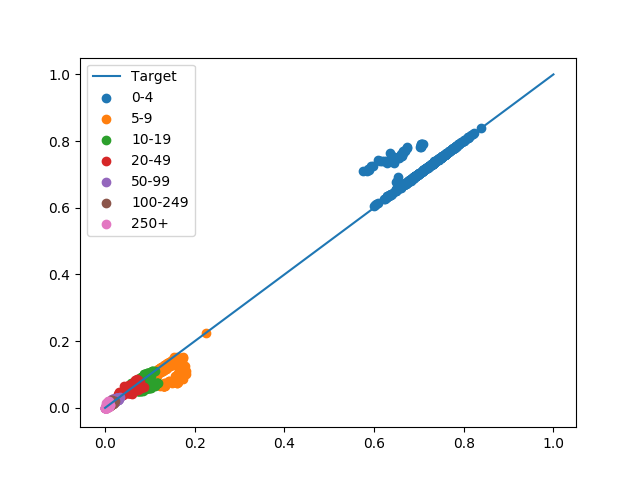
\includegraphics[width=\textwidth]{graphics/proportions_local_units}
 \caption{Analysis of Log Normal Distribution Fit - proportion in size bands predicted against actual}
 \label{ln_dist_fit}
 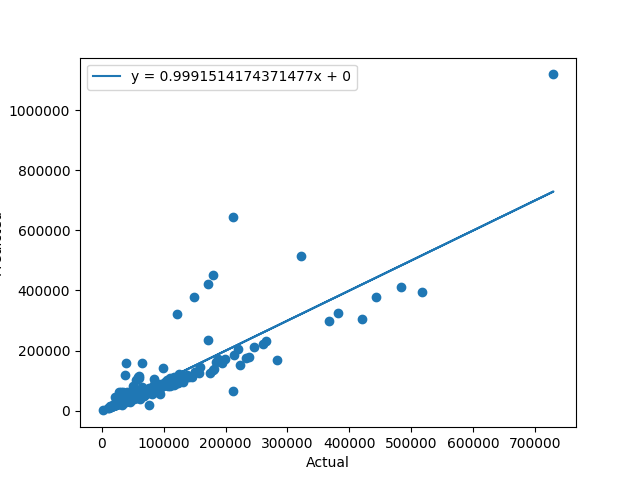
\includegraphics[width=\textwidth]{graphics/LA_employment_pred_locl_units}
 \caption{Prediction of employment per local authority - predicted against actual}
 \label{size_pred}
\end{figure}

Figure \ref{ln_dist_fit} shows that the lognormal distribution roughly approximates the size distribution of companies in each local authority and Figure \ref{size_pred} shows that the size prediction does a good job for most local authorities - although generally underestimating but for some local authorities the prediction is off by about $4 \times 10^5$ jobs which is an issue.

The same procedure can be done but using SIC codes and the distribution of sizes within each SIC code.
%TODO: Do this analysis

\section{Combining CH Granular Data with ONS reports}
Since the Companies House open data doesn't contain some of the most important properties of a company (number of employees and turnover in particular) we assign companies properties in a way that matches conditionally probabilistic growth models. The conditions being that the granular dataset reproduces the ONS aggregated statistics and that the companies die when the real CH companies die\footnote{Due to the lack of data, we have been unable to test the accuracy of this method of prediction}.
\subsection{Assumptions}

\begin{itemize}
 \item ONS data is accurate
 \item Each enterprise on the ONS report is a collection of Companies registered on CH
\end{itemize}

\subsection{Deciding the Combinations of CH Entities that make up Enterprises}
For this study we assumed that if a set of companies were all registered at the same address then they were part of the same enterprise. This could be an issue and we haven't looked into the decisions of where the registered office address of a company is. For example, it could be the case that certain companies handle their CH filings through some form of solicitors and the company ends up being registered with the solicitors rather than the company itself. In any case, the use of multiple addresses seems to be a good first approximation and helps to clean up the data - making the relationship between the number of companies and number of companies reported by ONS more linear.




\section{Results}

\subsection{Employment Migration Data and Visualization}
\subsection{Generating other ONS Data from Dataset}
\subsubsection{Employment totals}

\section{Structure of Dataset}
When dealing with highly granular data of this kind, a difficult question is how to store the data.

\end{document}
